\section{PD 内部分型特征扩展与权重敏感性分析}

考虑到 Healthy/PD 判别特征可能主要刻画疾病有无或总体异常程度，本文在 PD 受试者内部进一步构建分型特征方案，包括相关性去冗余、高 IQR/MAD 特征筛选和 SparsePCA 表示。为避免把解释便利性混入客观评价，推荐评分不对 Top20/Top50 设置额外奖励，也不把二类聚类与六类聚类的一致性作为六类方案的评分项。所有候选方案均在 Dataset 1 的 188 名 PD 受试者内部比较，不引入 Healthy 样本或记录级录音样本。

权重敏感性分析同时考虑 silhouette、Calinski-Harabasz、反向 Davies-Bouldin、稳定性 ARI 和簇均衡性五个指标，并随机生成 10000 组 Dirichlet 权重。每组权重下重新计算综合分并记录排名第一和排名前三的候选方案，由此判断推荐结论是否依赖某一组主观权重。

二类潜在语音表型采用多候选报告口径。\feature{top20_biomarkers} / \feature{pca_5} / KMeans 的 top-1 频率最高，为 37.3\%，但低于 60\% 的稳健主推荐阈值，因此作为相对推荐候选方案。与此同时，\feature{top50_biomarkers} / \feature{pca_5} / KMeans 和 \feature{pd_high_iqr_top50} / \feature{pca_5} / AgglomerativeClustering 也作为可接受候选同步报告。这一结果说明二类潜在语音表型对权重设定仍有一定敏感性，不宜写作唯一稳健最优。

六类潜在语音表型采用 \feature{top20_biomarkers} / \feature{pca_5} / AgglomerativeClustering 作为稳健主推荐方案。该方案 top-1 频率为 87.1\%，在无解释性奖励、无二类聚类一致性评分项的设定下仍达到稳健主推荐阈值。因此，本文将该方案限定表述为 \(k=6\) 潜在语音表型聚类，而不写作由临床症状标签监督得到的诊断模型。

\begin{table}[H]
\centering
\caption{二类潜在语音表型权重敏感性主要候选}
\begin{tabularx}{\textwidth}{lYcc}
\toprule
候选 & 特征 / 表示 / 聚类方法 & top-1 频率 & top-3 频率 \\
\midrule
1 & \feature{top20_biomarkers} / \feature{pca_5} / KMeans & 37.3\% & 63.2\% \\
2 & \feature{top50_biomarkers} / \feature{pca_5} / KMeans & 22.4\% & 35.2\% \\
3 & \feature{pd_high_iqr_top50} / \feature{pca_5} / AgglomerativeClustering & 21.0\% & 28.9\% \\
\bottomrule
\end{tabularx}
\end{table}

\begin{table}[H]
\centering
\caption{六类潜在语音表型权重敏感性主要候选}
\begin{tabularx}{\textwidth}{lYcc}
\toprule
候选 & 特征 / 表示 / 聚类方法 & top-1 频率 & 判定 \\
\midrule
1 & \feature{top20_biomarkers} / \feature{pca_5} / AgglomerativeClustering & 87.1\% & 稳健主推荐 \\
2 & \feature{all_acoustic} / \feature{pca_90} / GaussianMixture & 12.9\% & 可接受候选 \\
\bottomrule
\end{tabularx}
\end{table}

\begin{figure}[H]
\centering
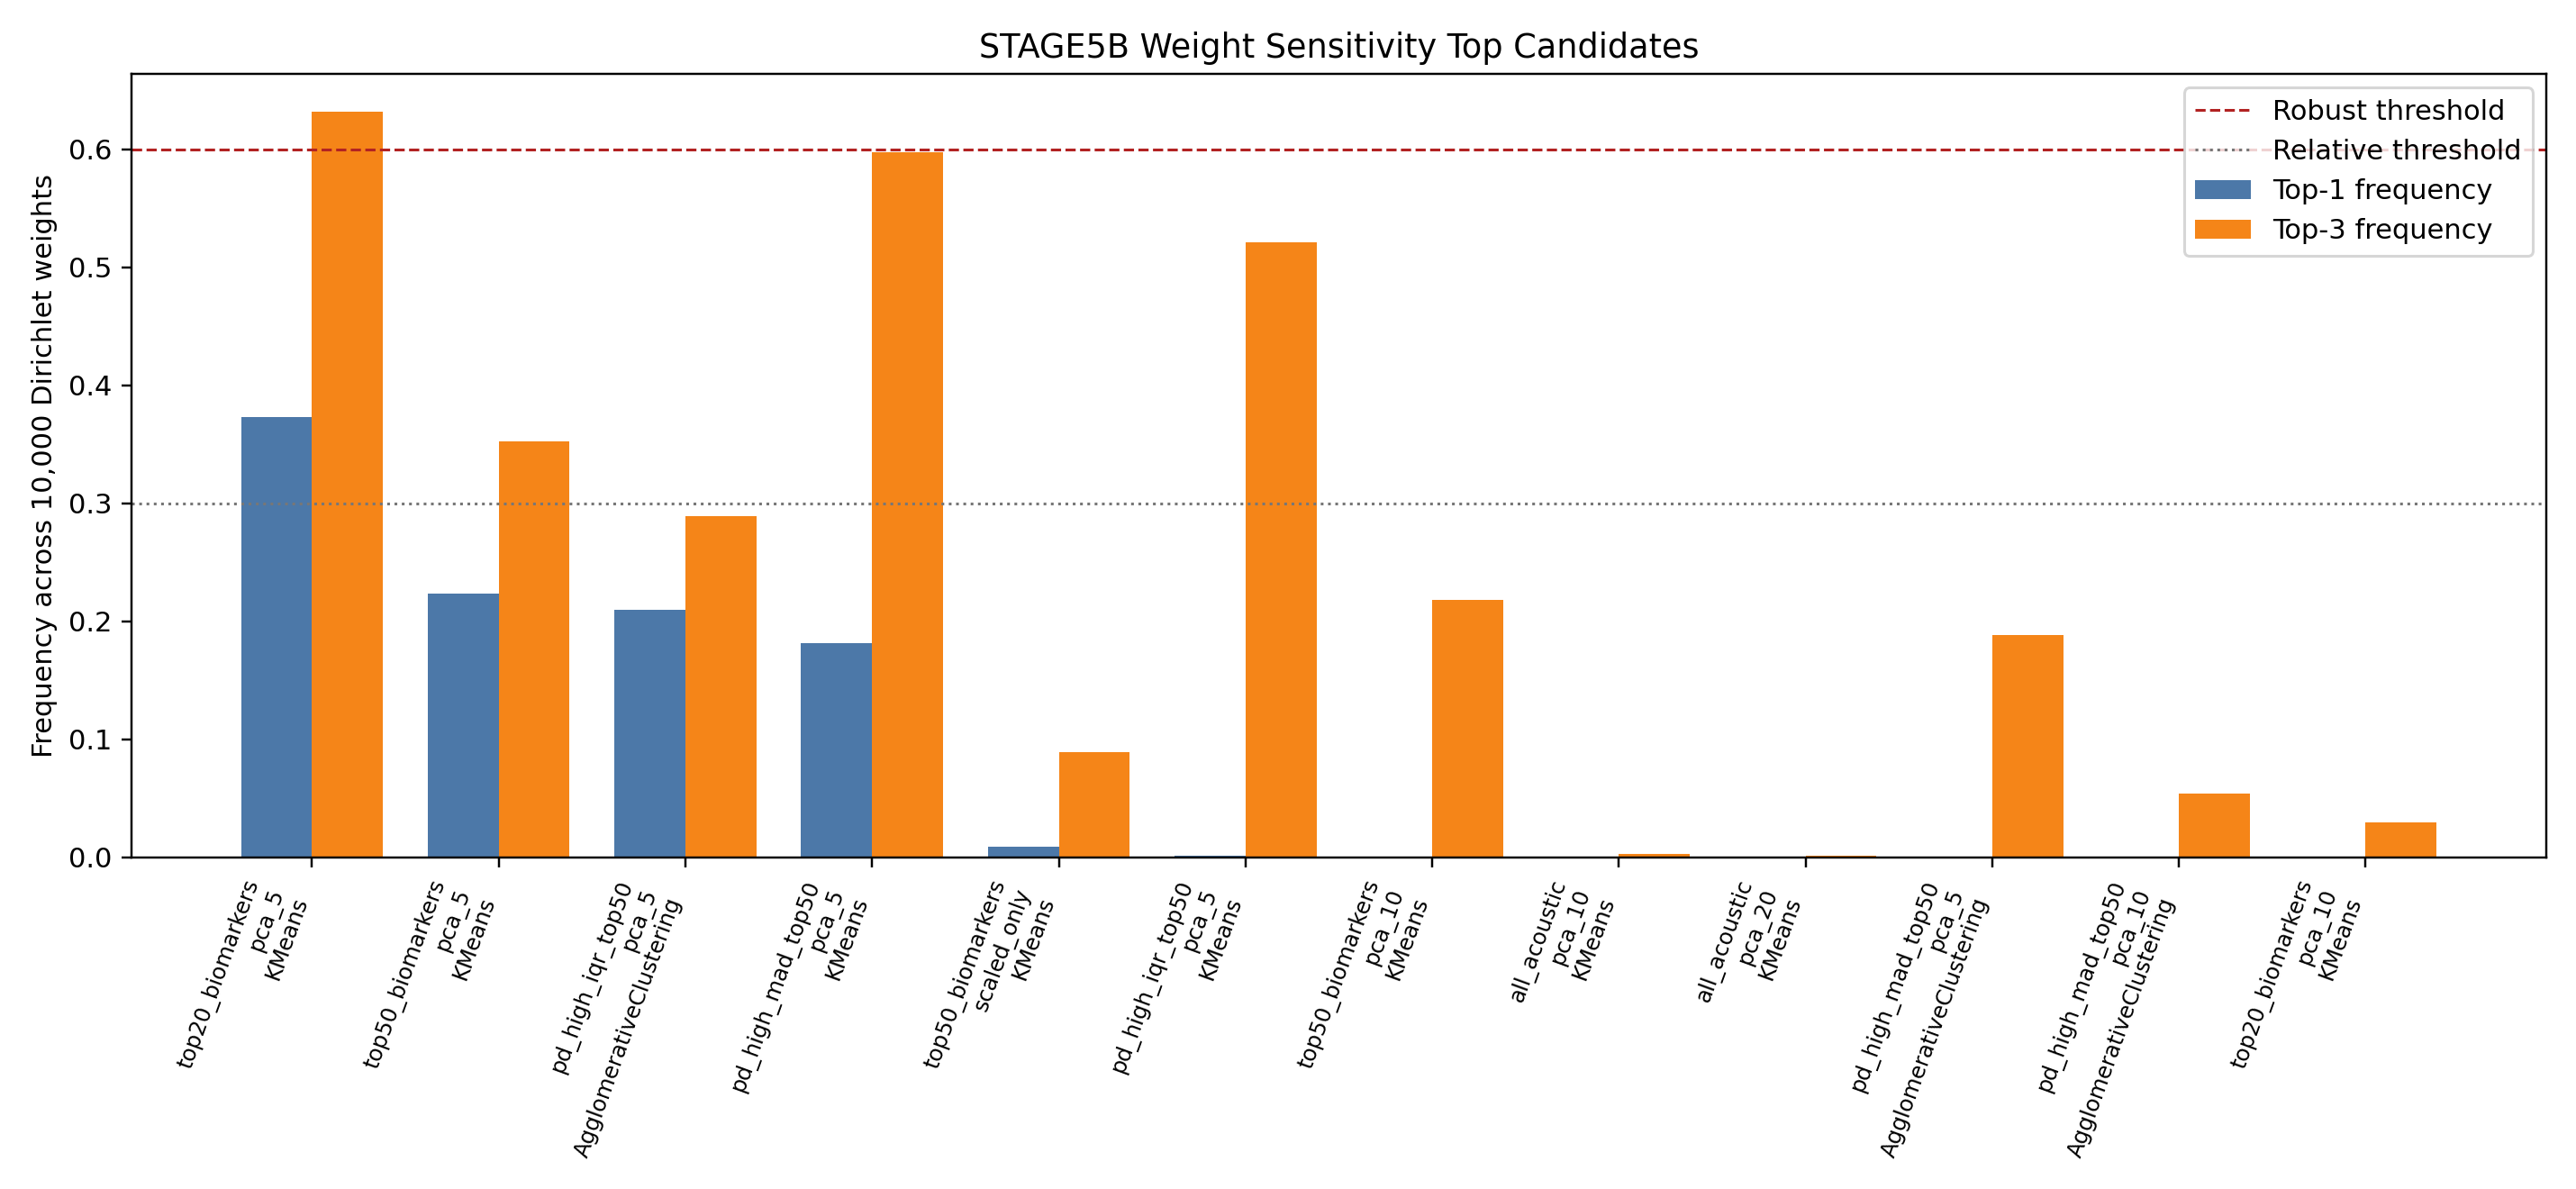
\includegraphics[width=0.88\textwidth]{figures/stage5b_weight_sensitivity_top_candidates.png}
\caption{二类潜在语音表型权重敏感性主要候选}
\end{figure}

\begin{figure}[H]
\centering
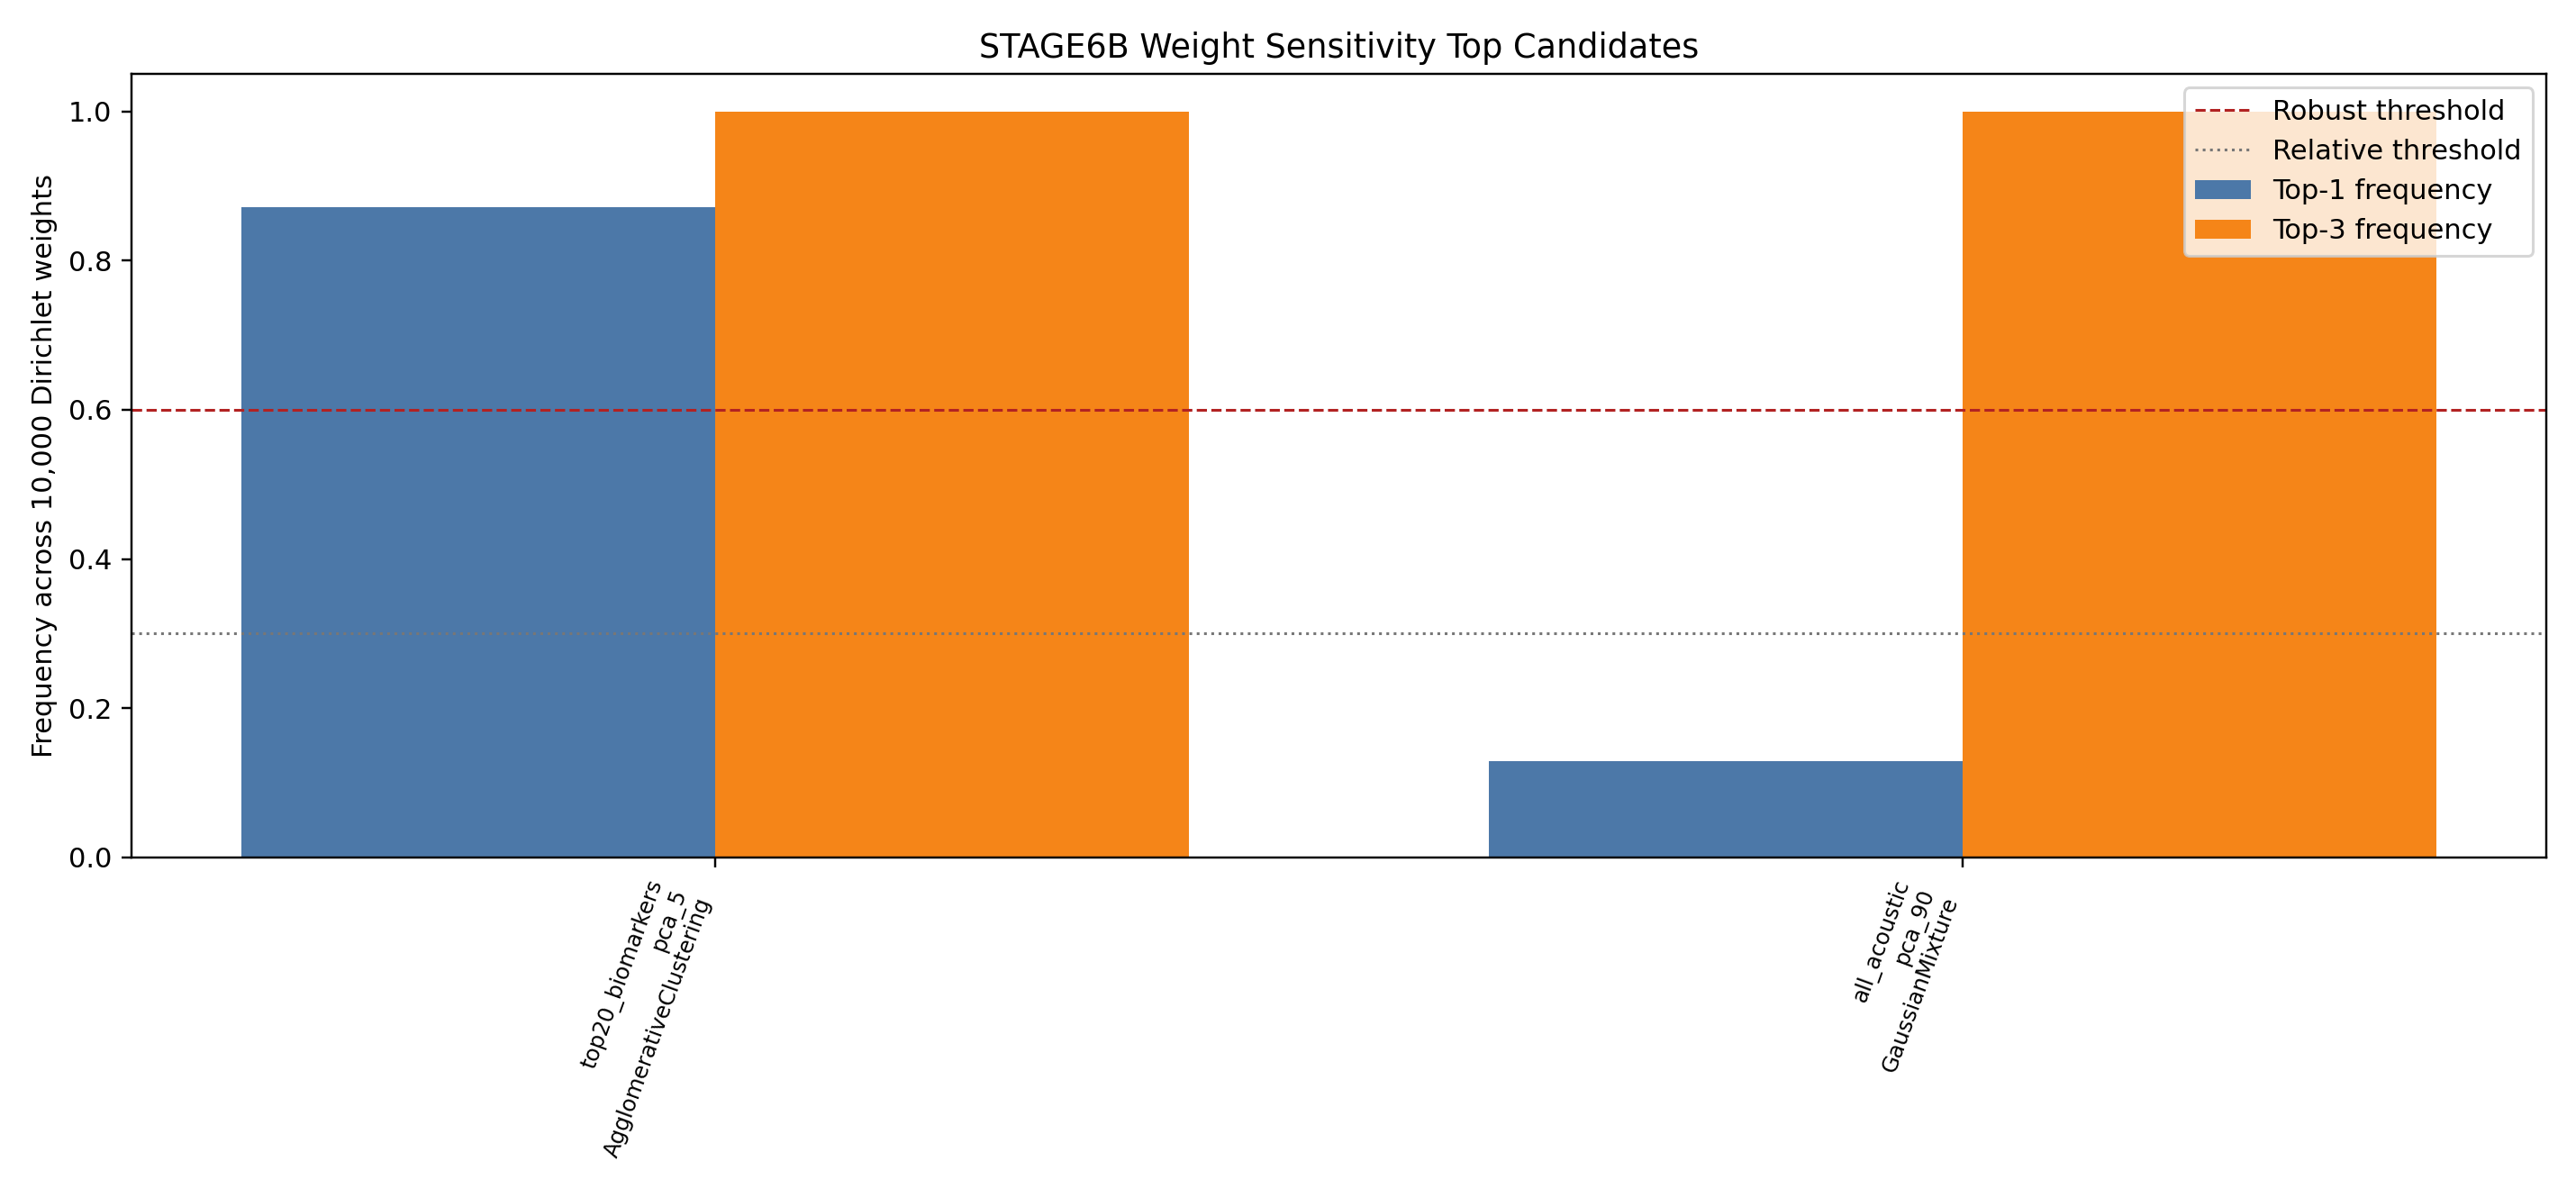
\includegraphics[width=0.88\textwidth]{figures/stage6b_weight_sensitivity_top_candidates.png}
\caption{六类潜在语音表型权重敏感性主要候选}
\end{figure}

综上，二类潜在语音表型结果采用“相对推荐候选方案 + 多候选并列报告”的表述；六类潜在语音表型结果采用“稳健主推荐方案”的表述，但严格限定为声学空间中的 \(k=6\) 潜在语音表型聚类。
